\section{Introduction}
In the field of robotics, platforms are of increasing importance. A platform is divided into a software platform and a hardware platform. There are a variety of features that make up robot software platforms, including low-level device control, SLAM (Simultaneous Localization and Mapping), navigation, manipulation, recognition of objects or people, sensing and package management, debugging and development tools, which are mostly used in the industrial sector where robot software platforms are currently primarily employed. Robot hardware platforms not only study platforms such as mobile robots, drones, and humanoids, but also commercial products. Hence, robot researchers from around the world are collaborating to discover a platform that is intuitive and open source. The most popular robot software platform is ROS, that means Robot Operating System. ROS, the Robot Operating System, is an open source framework to manage robots’ operations, tasks, motions, and other things. ROS is intended to serve as a software platform for those who build and use robots daily, but at the same time for people who are starting to use robots no long ago. This common platform allows newcomers to be increasingly inclined to read more and more and it is very easy to use. The design of the ROS platform allows the use of code and information shared by other programmers, which means you do not have to write all code in order to move the robots.
\newpage
\section{History of ROS}
“In May 2007, ROS was started by borrowing the early opensource robotic software frameworks including switchyard, which is developed by Dr. Morgan Quigley by the Stanford Artificial Intelligence Laboratory in support of the Stanford AI Robot STAIR (Stanford AI Robot) project.
Dr. Morgan Quigley is one of the founders and software development manager of Open Robotics (formerly the Open Source Robotics Foundation, OSRF), which is responsible for the development and management of ROS.
Switchyard is a program created for the development of artificial intelligence robots used in the AI lab’s projects at the time and it is the predecessor of ROS.
In addition, Dr. Brian Gerkey, the developer of the Player/Stage Project and 2D Stage simulator, later influence the growth of 3D simulator Gazebo, which was developed since 2000 and has had a major impact on ROS’s networking program. He is the co-founder of Open Robotics.
In November 2007, U.S. robot company Willow Garage succeeded the development of ROS. Willow Garage is a well-known company in the field of personal robots and service robots.” \cite{Quigley15}\\
Robots are computer-controlled electromechanical devices.
First dedicated robot programming languages arose in the 1970's.
There were robot-centric data types and some robot function libraries. They did not allow neither hardware abstractio, nor multi-robot interaction nor integrated simulation. There did not exist code reuse or standardization.
The efforts to build robot programming system continued through 80's, 90's and especially in the 2000's were there was a high push to standardize robot components, their interfaces and basic functions.\\
Hence, ROS as it is known today was initially developed in 2007 at the Standford Artificial Intelligence Laboratory. Since 2013 it is managed by OSRF and nowadays it is used by many robots, universities and companies, becoming the de facto standard for robot programming.
\begin{figure}[H]
    \centering
    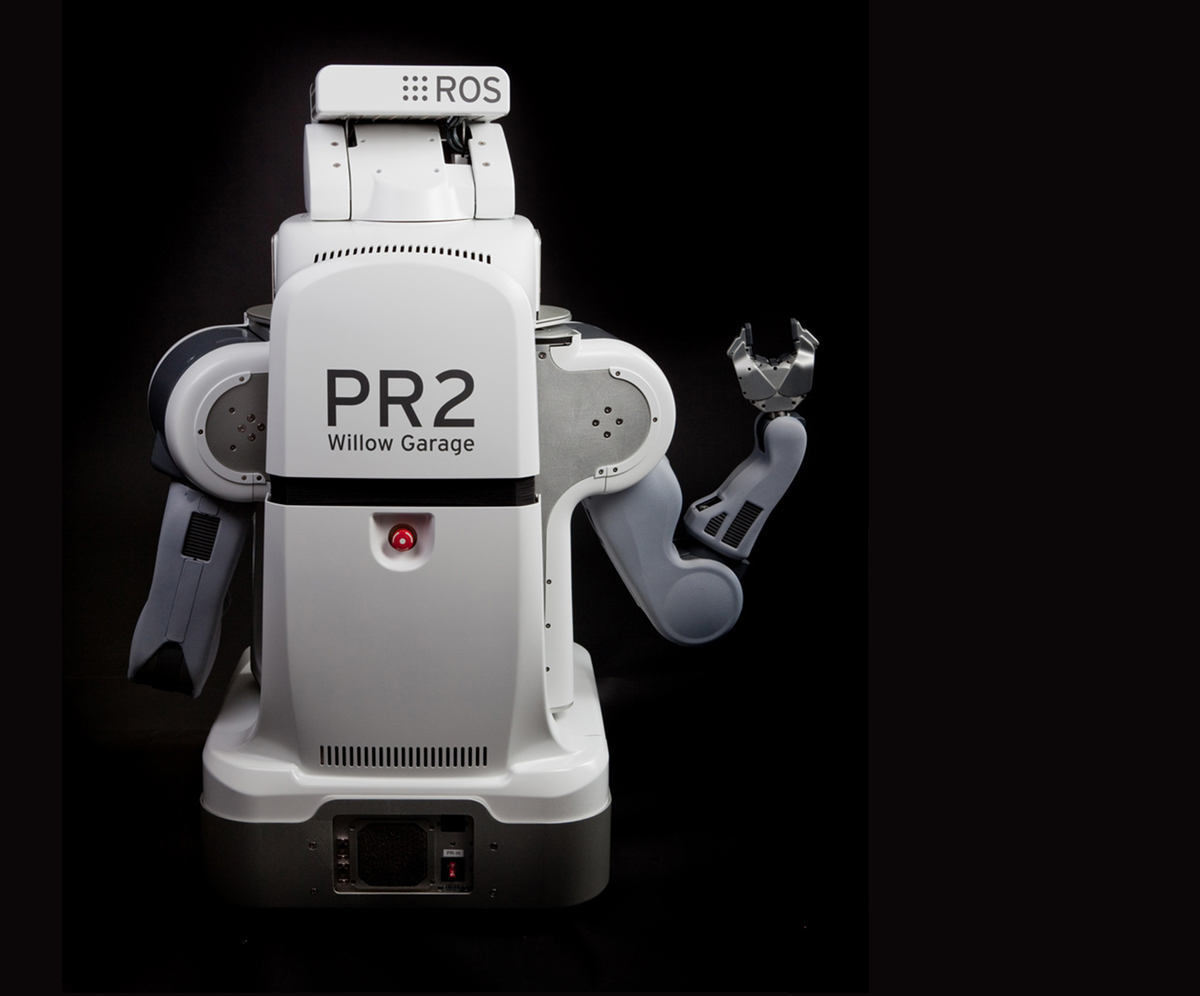
\includegraphics[scale=0.16]{Images/Chapter 1/PR2_Robot_Willow_Garage_6-1.jpeg}
    \caption{Willow Garage PR2 robot}
    \label{fig:PR2}
\end{figure}
\newpage
\section{Meta-Operating System}
ROS is an open source, meta operating framework for robots, hence it is nothing else than a middleware. \\
A middleware can be defined as a piece of software that gives an extra level of abstraction to the developer through a layer between the operating system and the applications.
It basically sits in the middle of software components and facilitates their interaction. \\
Its purpose is to provide an abstraction model for functions and at the same time provides the low-level implementation.
Every middleware must provide:
\begin{itemize}
    \item Portability: common programming model regardless the programming language and system architecture
    \item Complexity management: low-level aspects are managed by libraries and drivers inside the middleware itslef
    \item Reliability: middleware allows robot developer to discard low level details
    \item abstraction from sensors/actuators hardware;
    \item communication protocol for data transport
\end{itemize}
 As a result, they play an essential role in the development of complex applications that rely on a number of hardware and software tools.\\
 While they are still under active development, they are not yet capable of providing a complete set of functions for general purpose robots.
 
\begin{figure}[H]
    \centering
    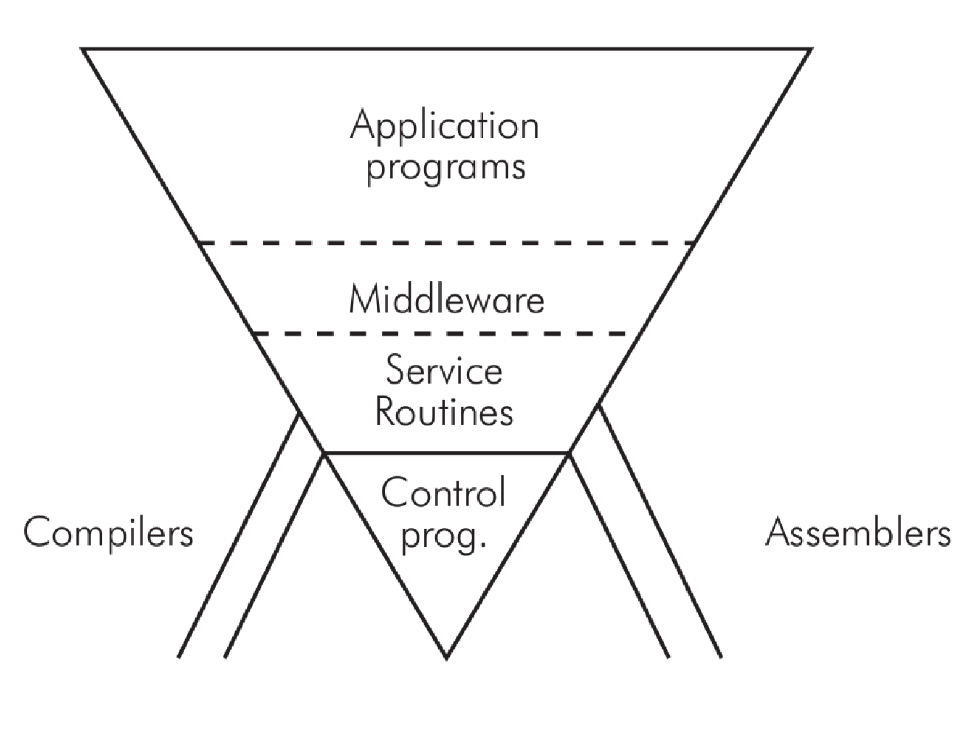
\includegraphics[scale=0.5]{Images/Chapter 1/middleware.png}
    \caption{Meta Operating System}
    \label{fig:metaoperating}
\end{figure}
 
 Several robotic middlewares have been proposed in the past years (OROCOS, ORCA, YARP, BRICS etc.) and eventually came ROS.
 
 \subsection{Phylosophy of ROS}
The following paragraphs describe some philosophical aspects of ROS:\\
\begin{itemize}
\item \textit{Peer to peer}: ROS systems consist of a small number of computer programs that are linked to one another and continuously exchange messages. These messages travel directly from one program to another. Although this makes the system more complex, the result is a system that balances better as the number of data increases.\\
\item \textit{Distributed}: Programs can be run on multiple computers and comunicate over the network.
\item \textit{Multilingual}: ROS chose a multilingual approach. ROS software modules can be written in any language for which a client library has been written. At the time of writing, client libraries exist for C++, Python, LISP, Java, JavaScript, MATLAB and others.\\
\item \textit{Thin}: the ROS conventions encourage contributors to create standalone libraries and then wrap those libraries, so that they can send and receive messages to and from other ROS modules. This extra layer is proposed to allow the reuse of software outside of ROS for other applications, and it greatly simplifies the creation of automated tests using standard continuous integration tools.\\
\item \textit{Free and open source}: the core of ROS is released under the permissive BSD license, which allows both commercial and non-commercial use. ROS foresees data exchange between modules using inter-process communication (IPC), which means that systems built using ROS can have fine-grained licensing of their various components.\\
\end{itemize}

\section{ROS Architecture}
ROS is based on a graph architecture where processing takes place in nodes, which communicate with each other by exchanging messages asynchronously through the use of topics to which they can subscribe to and/or on which they can publish, and synchronously with the calling of services, similar to RPCs.  Structurally, ROS is developed on 3 conceptual levels, File-system Level, Computational Level and Community Level, of which we are going to examine the constituent elements and their role in the architecture.
\subsection{File-system Level}
The Filesystem Level includes all resources used in ROS, in particular
\begin{itemize}
    \item Packages
    \item Metapackages
    \item Manifest
    \item Message types
    \item Service types
\end{itemize}
\begin{figure}
    \centering
    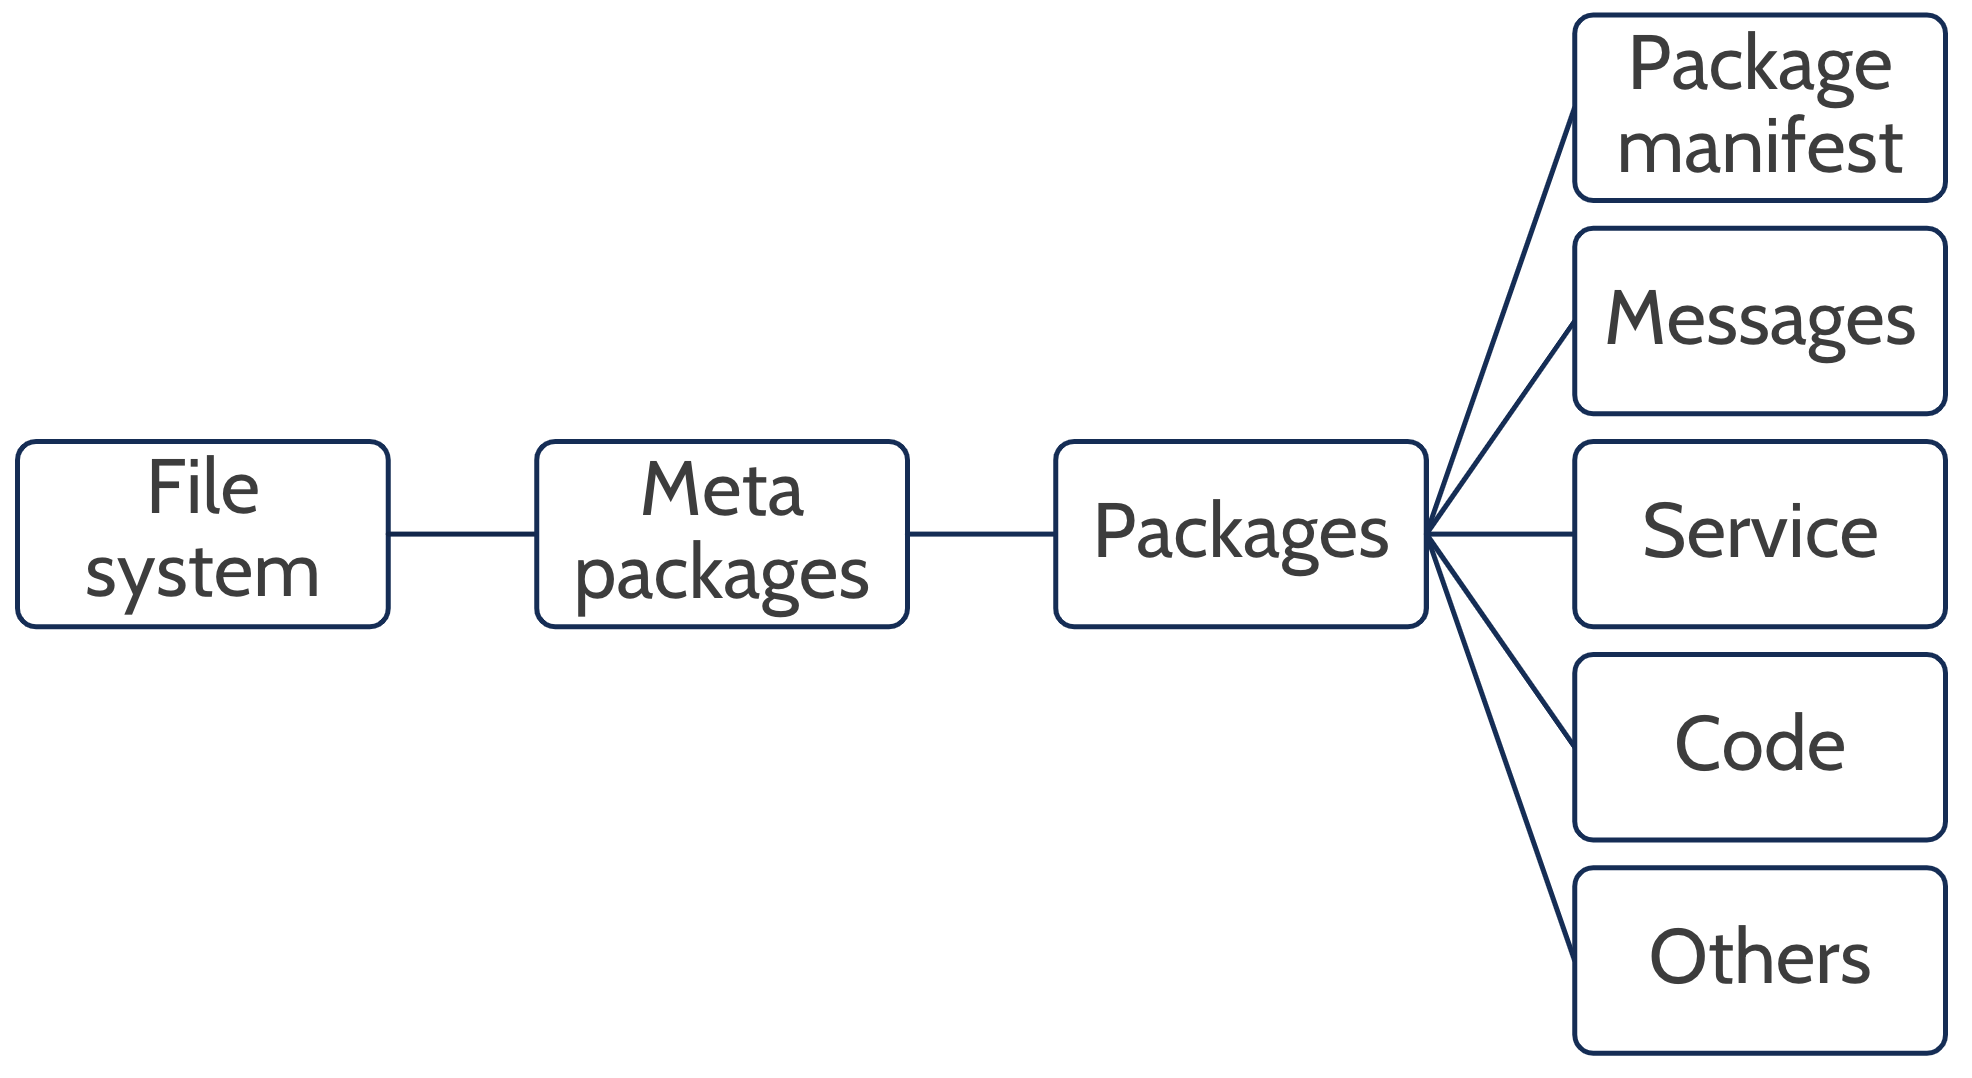
\includegraphics[scale=0.5]{Images/Chapter 1/Filesystem.png}
    \caption{File System level representation}
    \label{fig:Filesystem}
\end{figure}
\textbf{Packages}\\
Packages are the main structure for organising ROS  \citet{rospackages}. The processes, libraries, configuration files, datasets, and all the files used by the system at runtime are stored in these files. They are the structure that can be found within a ROS-based system. At the filesystem level, the package is represented by a directory. The structure within it includes some subfolders to manage the elements
In order to facilitate its development, in particular:
\begin{itemize}
    \item \textit{include/packagename}: C++ include headers (make sure to export in the CMakeLists.txt)
    \item \textit{msg}:Folder containing Message (msg) types
    \item \textit{src/packagename}: Source files, especially Python source that are exported to other packages.
    \item \textit{srv/}: Folder containing Service (srv) types
    \item \textit{scripts}: executable scripts
    \item \textit{CMakeLists.txt}: CMake build file
    \item \textit{package.xml}:XML file containing package structure 
    \item \textit{CHANGELOG.rst}: Many packages will define a changelog which can be automatically injected into binary packaging and into the wiki page for the package
\end{itemize}\\

\textbf{Metapackages}\\
Metapackages are specialised structures whose only task is to represent a group of packages that have common characteristics with each other. The metapackages that are created in the context of older versions of ROS and later updated may also result from the conversion of older stacks that perform similar functions in the context of older versions of ROS \citet{rosmetapackages}.\\
\newline
\textbf{Manifest}\\
A package manifest consists of an XML file named package.xml that must be included in the root folder of any catkin-compliant package. It contains information about the package, including its name, version number, authors, maintainers, and dependencies on other catkin packages. There is a strong similarity between this concept and the manifest.xml file used in the legacy rosbuild build system. System package dependencies are declared in package.xml \citet{rosmanifest}.\\
\newpage
There are a minimal set of tags that need to be nested within the <package> tag to make the package manifest complete.
\begin{itemize}
    \item \textit{<name>}: The name of the package
    \item \textit{<version>}: The version number of the package;
    \item \textit{<description>}: A description of the package contents;
    \item \textit{<maintainer>}: The name of the person(s) that is/are maintaining the package;
    \item \textit{<license}: The software license under which the code is released.
\end{itemize}
\textbf{Message types}\\
Message types define the structure of messages sent by ROS \citet{rosmsg}. Each file, with extension .msg, represents a different type of message. Within the file each line represents a message field. Each line, in turn, contains two columns: the first one for the data type of the field
(Int32/int (C++/Phyton), bool, string, time, etc.), the second for the name. It is possible to assign values to the fields within these le, in this case we speak of constants. Example of msg file (C++):

\textbf{Service types}\\
Service type are files that define the structure of request/response for ROS services \citet{rossrv}.
These are directly built upon the msg format to enable communication between nodes. They are stored in dedicated .srv files in the srv/ subdirectory of a package.
Example of srv file (C++):
\begin{lstlisting}[language=C++]
 bool add(beginner_tutorials::AddTwoInts::Request  &req,
             beginner_tutorials::AddTwoInts::Response &res)
    {
      res.sum = req.a + req.b;
      ROS_INFO("request: x=%ld, y=%ld", (long int)req.a, (long int)req.b);
      ROS_INFO("sending back response: [%ld]", (long int)res.sum);
     return true;
   }
\end{lstlisting}

\newpage

\subsection{ROS Computational Graph Level}
The Computation Graph is the peer-to-peer network of ROS processes that are processing data together. The basic Computation Graph concepts of ROS are nodes, Master, Parameter Server, messages, services, topics, and bags, all of which provide data to the Graph in different ways \citet{rosconcepts}.\\
\begin{figure}[H]
    \centering
    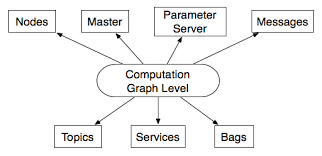
\includegraphics{Images/Chapter 1/computationgraph.png}
    \caption{Computation Graph}
    \label{fig:computationgraph}
\end{figure}
\textbf{Nodes}\\
A node is a process that performs computation. Nodes are combined together into a graph and communicate with one another using streaming topics, RPC services, and the Parameter Server \citet{rosnodes}. Following the concept of modularity of the system, each node will be related to only one specific functionality.\\ ROS in fact
discourages the creation of 'omnipotent' nodes that perform many functions in order to make the system more maintainable, reusable and clear.\\
The use of nodes in ROS provides several benefits to the overall system. There is additional fault tolerance as crashes are isolated to individual nodes. Code complexity is reduced in comparison to monolithic systems.\\
\newpage
\textbf{Topics}\\
Topics are buses identified by a proper and unique name that allow messages to be exchanged between nodes. They implement a mechanism
of publishing and subscribing: nodes can be publishers and/or subscribers if they are set up to send or receive messages. The division between
data producer and data user is clear and separated by anonymity policies
between the nodes. Each topic may have a maximum number of messages to be kept
in the queue in case they accumulate, those in excess are not added to the queue and lost \citet{rostopics}.\\
\newline
\textbf{Services}\\
Services are a two-way communication tool between nodes. It is a mechanism that extends that of messages with the possibility
not only to send commands to a specific node but also to remain in
listening and receiving a structured response from it. Each service is
first described in an .srv file where the parameters and type of service are indicated in addition to the name of the service.
of the service, as well as the parameters and the type of return data (see Service type).
Within the server node, the service is represented by a function
which takes as input two pointers to objects of the server class: one
one will include the function parameters (Request), the other will collect the return value.
will collect the return value \citet{rosservice}\\
\newline
\textbf{Messages}\\
The nodes in the graph communicate by exchanging messages. These
may be simple and of a primitive type (integer 
oat, string, char, etc.)
or arrays or even more complex, with structures similar to those seen in
C.\\
\newline
\textbf{Bags}\\
Bags represent the system by which ROS saves logs and keeps track of
all messages exchanged within a topic. The rosbag tool, once
associated with a topic, saves each message exchanged within a related file with the extension .bag. It is
very useful for storing data from the
sensors as it allows the developer to create a sort of "black box" of the robot.
black box" of the robot. ROS also provides a playback tool that allows the
visualise and playback the collected data via a graphical interface.\\
\newpage
\textbf{Master}\\
The master in ROS first takes care of registering new nodes within the
network, then managing the connection between the nodes in the graph, routing
messages and allowing access by one node to the services of another.
It is the heart of the software and can only be active one master at a time. It can be started via the roscore command or launched automatically
at the start of a node through the correct implementation of the file.
\begin{figure}[H]
    \centering
    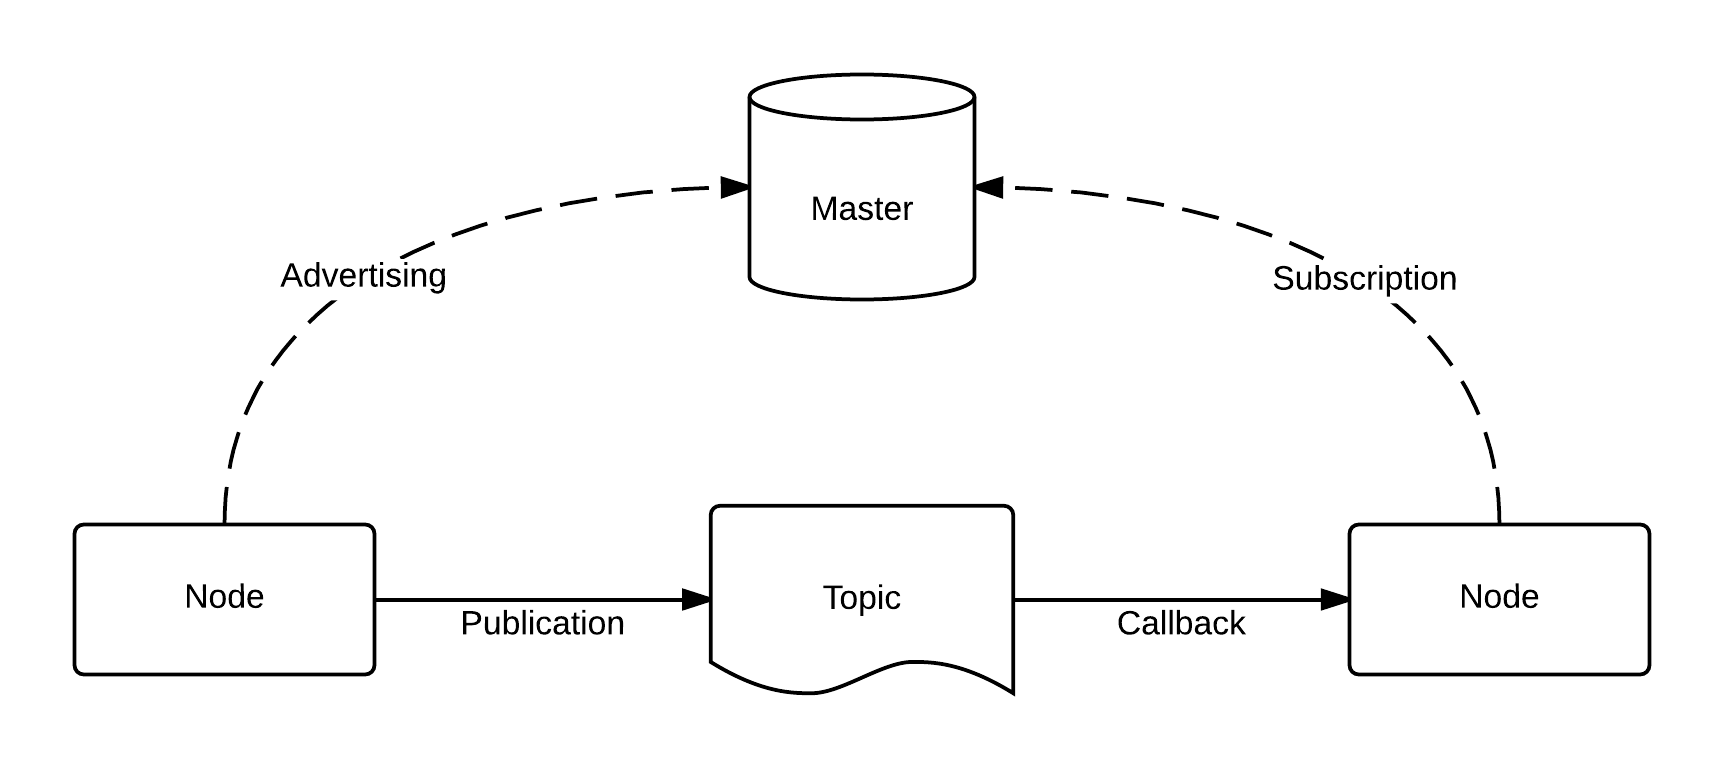
\includegraphics{Images/Chapter 1/ROS-master-node-topic.png}
    \caption{Visualization of Master-Node-Topic relationship}
    \label{fig:master-node-topic}
\end{figure}
\\
\newline
\textbf{Parameter server}\\
The parameter server is basically a component of the master, allowing certain configurations accessible via the network API to be shared publicly with all nodes. Although not an extremely high-performing it is nevertheless useful for the testing phase of the software. Parameters are named using the normal ROS naming convention. This means that ROS parameters have a hierarchy that matches the namespaces used for topics and nodes, \citet{rosparmserv}.